\documentclass{article}
\usepackage{geometry}
\usepackage{fancyhdr}
\usepackage[pdftex]{graphicx}
\usepackage{cite}
\usepackage{listings}
\usepackage{caption}
\usepackage{color}
\usepackage{underscore}
\usepackage{url}

  \usepackage{courier}

% from http://stackoverflow.com/questions/741985/latex-source-code-listing-like-in-professional-books
 \lstset{
         basicstyle=\footnotesize\ttfamily, % Standardschrift
         numbers=left,               % Ort der Zeilennummern
         numberstyle=\tiny,          % Stil der Zeilennummern
         %stepnumber=2,               % Abstand zwischen den Zeilennummern
         numbersep=5pt,              % Abstand der Nummern zum Text
         tabsize=2,                  % Groesse von Tabs
         extendedchars=true,         %
         breaklines=true,            % Zeilen werden Umgebrochen
         keywordstyle=\color{red},
            frame=b,         
%        keywordstyle=[1]\textbf,    % Stil der Keywords
%        keywordstyle=[2]\textbf,    %
%        keywordstyle=[3]\textbf,    %
%        keywordstyle=[4]\textbf,   \sqrt{\sqrt{}} %
         stringstyle=\color{white}\ttfamily, % Farbe der String
         showspaces=false,           % Leerzeichen anzeigen ?
         showtabs=false,             % Tabs anzeigen ?
         xleftmargin=17pt,
         framexleftmargin=17pt,
         framexrightmargin=5pt,
         framexbottommargin=4pt,
%         showstringspaces=false      % Leerzeichen in Strings anzeigen ?        
 }

\DeclareCaptionFont{white}{ \color{white} }
\DeclareCaptionFormat{listing}{
  \colorbox[cmyk]{0.43, 0.35, 0.35,0.01 }{
    \parbox{\textwidth}{\hspace{15pt}#1#2#3}
  }
}
\captionsetup[lstlisting]{ format=listing, labelfont=white, textfont=white, singlelinecheck=false, margin=0pt, font={bf,footnotesize} }

\newcommand{\code}[3]{
\lstinputlisting[
firstnumber=#1,
firstline=#1,
lastline=#2,
caption=#3
]{../oeving1.s}
}

\newcommand{\codewithfile}[4]{
\lstinputlisting[
firstnumber=#1,
firstline=#1,
lastline=#2,
caption=#3
]{#4}
}

%TCIDATA{OutputFilter=LATEX.DLL}
%TCIDATA{Version=5.50.0.2953}
%TCIDATA{<META NAME="SaveForMode" CONTENT="1">}
%TCIDATA{BibliographyScheme=Manual}
%TCIDATA{Created=Monday, January 30, 2012 17:20:46}
%TCIDATA{LastRevised=Monday, February 27, 2012 12:06:08}
%TCIDATA{<META NAME="GraphicsSave" CONTENT="32">}
%TCIDATA{<META NAME="DocumentShell" CONTENT="Standard LaTeX\Blank - Standard LaTeX Article">}
%TCIDATA{CSTFile=40 LaTeX article.cst}

\newenvironment{proof}[1][Proof]{\noindent\textbf{#1.} }{\ \rule{0.5em}{0.5em}}

% Sets page margins to 1", which is standard
\geometry{left=1in,right=1in,top=1in,bottom=1in} 

% allows the included extensions of graphic files
\DeclareGraphicsExtensions{.pdf,.png,.jpg}

% sets/adds graphic path. If empty it just looks around the folder the .tex file is in
\graphicspath{{}}

% I do not remember what this does
\setlength{\headheight}{15.2pt}

% allows the xhead parameters
\pagestyle{fancy}

% Sets the left header
\lhead{Group \#10}

% Sets the right header
\rhead{Lab Assignment \#3, TDT4258 Spring 2013}

% everything before this is considered the header or whatever.
\begin{document}

% INCLUDEGRAPHICS EXPLANATION
% \includegraphics[scale=1]{name of file}
% sometimes you want to twice encase the filename in squiggly brackets. I do not know why but sometimes it is required.

% begin title page, use \\ for newline
\title{Report from Lab Assignment \#3\\TDT4258 Energy Efficient Computer Systems}

% now one can list the authors, \textbf{} makes bold text
\author{Emil Taylor Bye\\Sigve Sebastian Farstad\\Odd M. Trondrud}

\pagenumbering{roman} 

% make title page
\maketitle


\bigskip
\bigskip
\bigskip
\bigskip

\part*{Abstract}

This report presents a solution to assignment \#3 of TDT4258 at the Norwegian University of Technology and Science during the spring of 2013.
The assignment was to write a video game in C for Linux running on the Atmel STK1000 development board.
Linux Device Drivers for the STK1000's buttons and LEDs were written in C.
The solution presented in this report is a rhythm video game, implementing the .SM file format.

\newpage

\tableofcontents

\setcounter{secnumdepth}{3}

\newpage 

\setcounter{page}{1}
\pagenumbering{arabic} 

\part{Introduction}

This report presents a solution to assignment \#2 of TDT4258 at NTNU, during the spring of 2013.
The objective of this lab assignment is to write a program in C for the STK1000 development board which causes different sounds to play when different buttons on the board are pressed, using an interrupt routine to pass the audio samples to the board's ABDAC (Audio Bitstream Digital to Analog Converter).
A minimum of three different sound effects should be made, as well as a ``start up melody''.

This report details the development of the sound-generating program as a solution to the assignment.
\section{The STK1000}
	The STK1000 is a development board from Atmel which offers a complete development environment for Atmel's AT32AP7000 processor.
	It offers a multitude of different peripheral I/O devices, of which this assignment will be using an array of LEDs and some push buttons.
	The processor is an ARM32 processor, and will for this assignment be only running the assembled output of hand-coded C code, without the support of an operating system.

\section{A note on sound}
	In order to write a program to generate sound, one should first study the physical properties of sound, and research different strategies to generate sound in a digital environment.

Sound is a mechanical wave that is an oscillation of pressure composed of frequencies within the range of hearing\footnote{http://en.wikipedia.org/wiki/Sound}.

Humans can percieve sounds with frequencies that range from about 20Hz - the lowest of basses - to 20kHz - the highest of high-pitched whining.
Sound is inherently analog, and requires some form of digital representation to be able to be generated by the AP7000, which is a digital device.
Regarding a sound wave as a continuous signal representing wave amplitude with respect to time, one straight-forward way of representing a sound wave digitally is to simply have an list of integer signal samples at a fixed, preferrably small, time interval.
This is indeed the format the AP7000 expects for its digital-to-analog converter.

There are different strategies available for preparing the stream of integers that needs to be sent to the digital-to-analog converter to generate a sound.
One strategy is simply to store the prepared list of integers somewhere in memory, and then copy it over to the DAC integer by integer as they are consumed by the ABDAC.
This strategy is analogous to rasterized bit maps in the image world.
This strategy, while easy to implement, and is able to represent all kinds of sounds, requires a great deal of memory (integer size * sample rate of bytes per second, in fact).
As an example, a three minute song, when stored at 16 bits per sample at a generously low sample rate of 22050Hz, requires 16 bits/sample * 180 seconds * 22050 samples/second = ̃ca 7.57 megabytes.
To put this in perspective, the entire flash memory of the AP7000 is 8 megabytes.
On a low memory platform like the STK1000, this is therefore not a great strategy.

Another strategy is the generative approach.
This strategy is analogous to vector based images in the image world.
The idea is to generate samples at run-time based on configurations read from memory, rather than reading the pre-generated values from memory.
This is a more CPU-hungry approach, but requires less memory than the previous strategy.
This strategy is used for the sound effect synth in the presented solution program.

A third strategy is a hybrid approach, where small sample lists are pre-bundled with the program, and generative rules are used to play back the samples at different times with different parameters.
This is the approach used in the music player in the presented solution program.



\section{About the MOD file format}
	The MOD file format is an old music tracker file format originally created for the Commodore Amiga (figure \ref{img-amiga}), a series of computers from the late eighties.
\begin{figure}[H]
	\caption{The Amiga 1000 (1985), the first Amiga model released. Image courtesy of Kaiiv.}
	\centering
	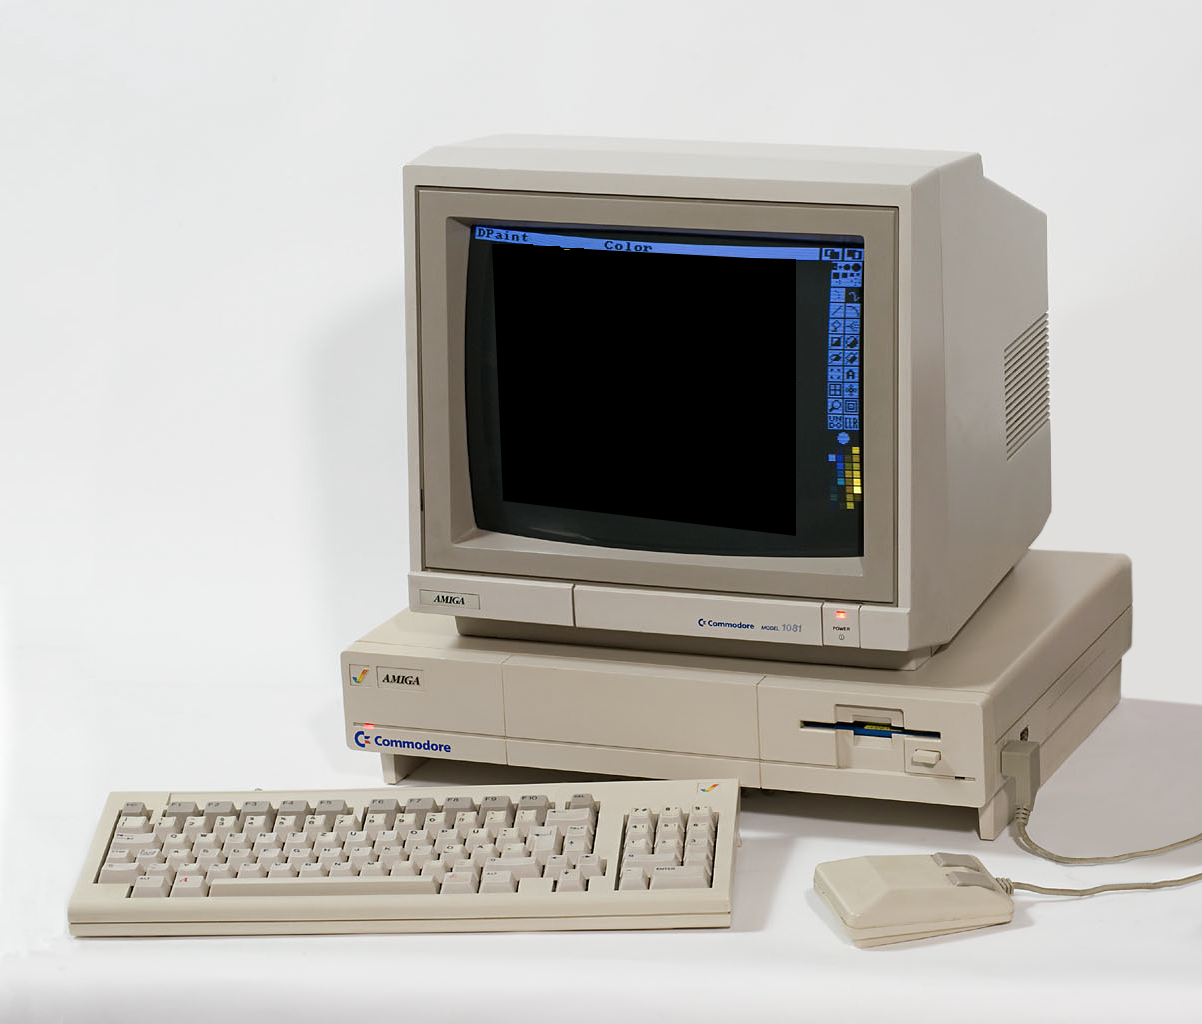
\includegraphics[width=4in]{{images/Amiga.jpg}}
    \label{img-amiga}
\end{figure}

The file format is tightly optimized for playback on the Amiga's audio hardware, so to understand the inner workings of the MOD file format, one should first know a little about how the Amiga's audio hardware works.

The Amiga's sound chip, called Paula, is capable of powering four simultaneous DMA-driven 8-bit PCM sample sound channels.
Each of these channels can be independently set to different sample frequencies many times per second.
The MOD format exploits this -- it supports 4 simultaneous channels of sample playback, using the frequency modulation to change the pitch of the samples played in the different channels.

Internally, the music in a MOD file is stored as a set of PCM-coded predefined sounds, as well as a large table of note patterns containing information about which sounds should be played at which frequencies and at which time.
The MOD format also includes a large set of musical effects such as tremolo, vibrato, arpeggio, portamento and so on, a subset of which are implemented in the presented solution program.

The MOD file format is not a defined standard, and does therefore not have a formal specification.
The MOD format grew organically from the early Amiga demoscene in the eighties, so many different variants exist -- each with with their own specialities and quirks.
The MOD Player presented in the solution is tailored to read so-called \texttt{M.K.} MODs generated by a MOD creator program (``tracker'') called ProTracker.
These MOD files are called \texttt{M.K.} MODs because they contain the magic number \texttt{M.K.} in the file header.
This is one of the most popular MOD formats, and has become a sort informal standard amongst MOD trackers.

\texttt{M.K.} MODs can have a maximum of 31 bundled PCM-coded sounds, 128 patterns, each with 64 note divisions for each of the four channels, and a a 128 item long list of which patterns should be played in what order.

Figure \ref{img-protracker} shows an image of a MOD file being edited in a tracker program.
Each column represents one channel, and each row represents one of the 64 divisions of a pattern.
The currently played division is traditionally kept vertically centered in the middle of the screen, as in this image.


\begin{figure}[H]
	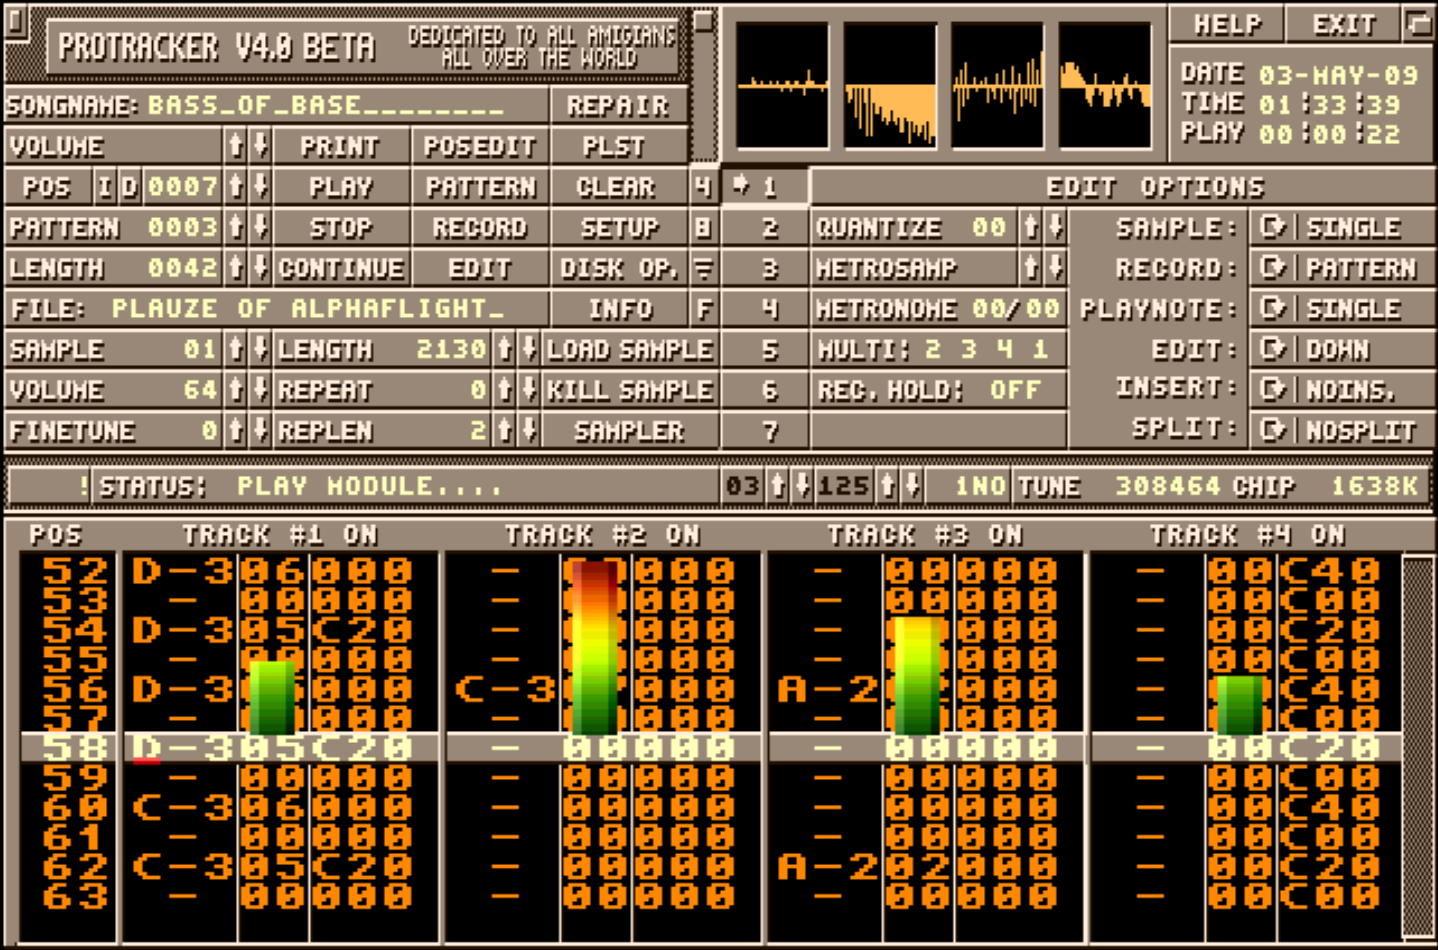
\includegraphics[width = \textwidth]{images/Protracker.png}
	\caption{A four-channel MOD being played in ProTracker. Image courtesy of Alec Graggamoor.}
	\label{img-protracker}
\end{figure}

These four resources do a pretty good job of documenting the MOD file format in detail:
\begin{itemize}
	\item{\url{http://www.mediatel.lu/workshop/audio/fileformat/h_mod.html}}
	\item{\url{http://archive.cs.uu.nl/pub/MIDI/DOC/MOD-info}}
	\item{\url{https://bel.fi/alankila/modguide/}}
	\item{\url{http://16-bits.org/mod/}}
\end{itemize}

\newpage


\part{Description and Methodology}

This section describes how the paddle program was developed.
It covers setup and configuration, tools and program details.

\section{Experimental Procedure}
    
    The first thing we did was locate the lab, on the fourth floor of the IT-Vest building, room 458. 
We removed one of the AVR32STK1000 boards from their box and set the jumpers to the appropriate positions (\cite{lab-compendium}, pg 37).
We booted up one of the computers and connected the AVR32STK1000 to it. 
Our first piece of code simply enabled all the LEDs and turned them on. Once we got the LEDs working we enabled the buttons.
We followed this up by writing code to turn on just one of the LEDs, designated the ''paddle'' per the assignment's description (\cite{lab-compendium}, pg 37).
Shortly thereafter we gave up on trying to figure out GDB.
Code was written to move right when \texttt{SW0} is pushed, and left when\texttt{SW2} is pushed, employing arithmetic shift to move the paddle bit in the appropriate direction.
However, a single push of either button caused the paddle to disappear, due to a combination of us simply letting the paddle's bit overflow when it reached either edge and the \emph{bouncing effect} (\cite{lab-compendium}, pg 22). We altered our code so that the paddle would ''loop around'' to the opposite side of the row of LEDs when it is ''pushed off'' either side.
When pushing either buttons, all the LEDs would light up briefly in turn at such high a speed that it looked like they were all lit simultaneously, again due to the bouncing effect.
Implementing debouncing (\cite{lab-compendium}, Fig. 2.9a) seemed like the next logical step, so the next thing we did was change our program to an interrupt-based solution.
Then we implemented debouncing.

We had an issue where the paddle would move over one additional LED when either button was pushed (i.e. from \texttt{LEDn} to \texttt{LEDn+2} rather than from \texttt{LEDn} to \texttt{LEDn+1}), which we fixed by, in effect, ignoring every second registered push of either buttons.
Finally we measured the current on the board's various pins while an interrupt-based program was running, and again with a busy-waiting program in order to compare the energy efficiency of the two solutions.


\section{Configuration of the STK1000}

    \subsection{Jumpers}

        The STK1000 has 10 jumpers that can be set to configure the board.
For this assignment the jumpers were set as specified on page 37 in \cite{lab-compendium}.


   \subsection{GPIO connections}

        The STK1000 provides a general purpose input/output interface (\texttt{GPIO}) with 32 signal lines.
16 of the 32 available lines were connected to on-board I/O devices on the STK1000 in this assignment.
The I/O devices in use were 8 on-board LEDs, used as a rudimentary paddle display, and 8 on-board switches, used as player controls.

The buttons were connected to \texttt{GPIO0-GPIO7} (\texttt{J1} on the STK1000) using a flat cable as in figure \ref{flat-cable-image}. This maps the buttons to ports \texttt{0-7} of \texttt{PIOB}.
The choice of low port numbers \texttt{0-7} is convenient for coding, and the choice of \texttt{PIOB} as opposed to \texttt{PIOC} is purely mnemonic ('B' for buttons).

The LEDs were connected to \texttt{GPIO16-GPIO23} (\texttt{J3} on the STK1000) using a flat cable as in figure \ref{flat-cable-image}. This maps the LEDs to ports \texttt{0-7} of \texttt{PIOC}.
Having the same port numbers for the buttons and the LEDs is a nice convenience for cleaner and more efficient code, as translation from button ports to LED ports is not necessary.

\begin{figure}
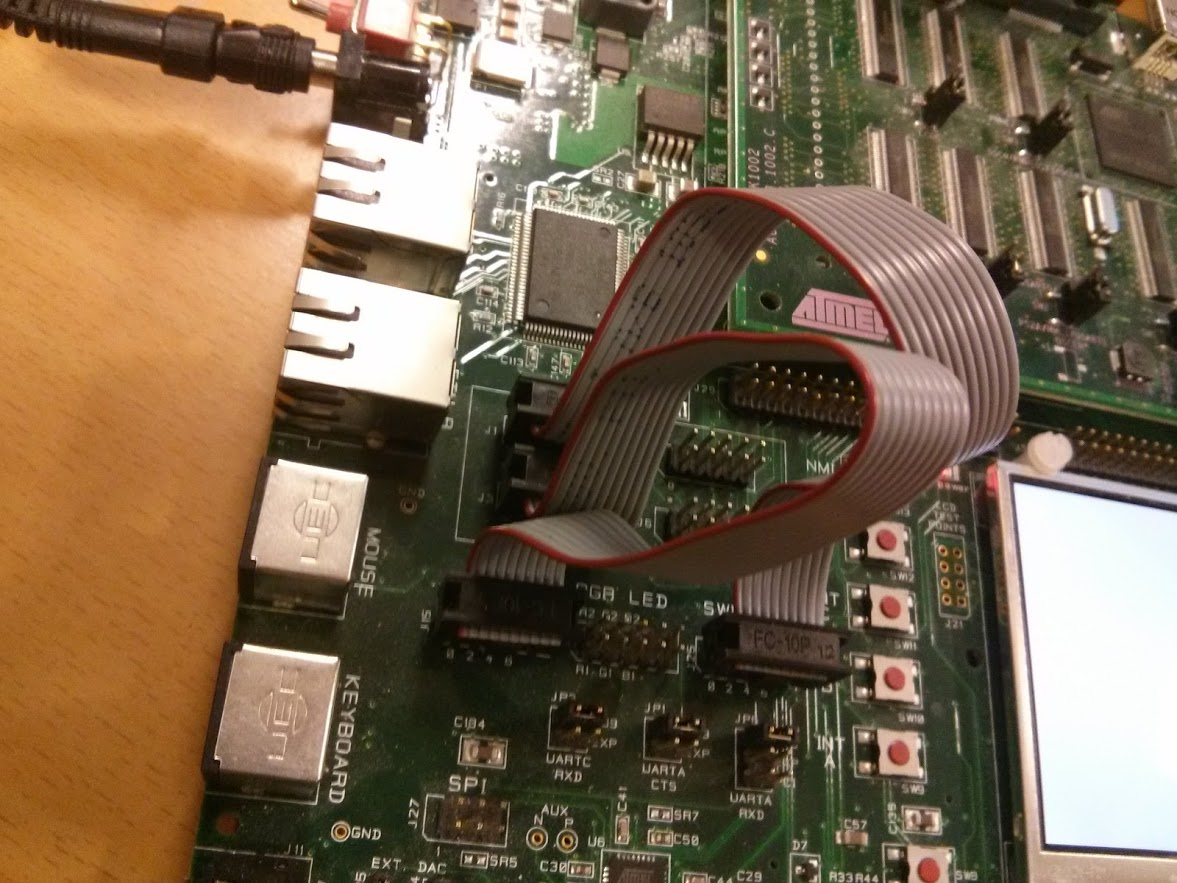
\includegraphics[width = \textwidth]{description-and-methodology/flat-cable-image.jpg}
\caption{Flat cables connecting GPIO with switches and LEDs. Note the orientation of the flat cables.}
\label{flat-cable-image}
\end{figure}


\section{Programming environment}

    \subsection{JTAGICE}

        The AP7000 sisterboard on the STK1000 provides a JTAG interface, which is used for programming and debugging of the board.
The development PC was connected to the JTAG interface of the STK1000 using an Atmel JTAGICE mk II (firmware 7.29).
The JTAGICE does not require external power as long as it is connected to the PC over USB.


    \subsection{GNU Debugger}
    % Done.
        We followed the instructions presented in the compendium in an attempt to employ the GNU debugger, but were confused by the interface as we had not read the recommended further reading material supplied in the compendium.
So we chose to not employ the GNU debugger in the development of our solution.
TODO: run up to the lab and use gdb a bit, so we can write about it here afterwards.


    \subsection{Make}

        GNU Make, a scriptable build tool, was employed in the development of the paddle program.
The handout files included a samle Makefile, which was used mostly without modification.
After the development of the program was complete, and how to use the debugger became clear (see the previous section), a make command to quickly enter debug mode was included.
This command could be invoked by writing \texttt{make debug}.
Aditionally, and somewhat self-referentially, a Makefile for easy compiling of this LaTeX report was used.


    \subsection{Other tools}

        vim, git.


\section{Development of the program}

This section details the steps taken during the development of the program.
Initially, a bare-bones program was developed with minimal functionality, to get familiar with the environment.
Features were added iteratively, starting with simple LED and button integration, and moving on to more sophisticated interrupt-oriented logic/program flow.

    \subsection{Setting up the LEDs}
        
        The connection to the output LEDs must be set up before the LEDs can be used in a program.
First, the I/O pins that the LEDs are connected to must be enabled.
In this assignment, the LEDs are connected to the pins GPIO16-23, corresponding to PIO C lines 0-7.
To enable the correct I/O pins, we must therefore set to 'high' bits 0-7 of the PIO C PIO Enable Register (PIOC PER), as in listing x.
Here, r3 is the base offset of PIOC, AVR32\_PIO\_PER is the PIO Enable Register offset, and r6 contains the bitfield indicating which pins to enable.

\code{99}{100}{Enable the I/O pins}

Second, the I/O pins must be set to act as output pins, as opposed to input pins.
This is done by setting to 'high' the corresponding bits (0-7) of the PIO C Output Enable Register (PIOC OER), as in listing x.
Here, r3 is the base offset of PIOC, AVR32\_PIO\_OER is the Output Enable Register offset, and r6 contains the bitfield indicating which pins to set as outputs.

\code{102}{103}{Set the pins to act as output pins}

Once this is done, LEDs can be turned on by writing the appropriate bits to PIO C Set Output Data Register (PIOC SODR), as in listing x.
Here, r3 is the offset of PIOC, AVR32\_PIO\_SODR is the Set Output Data Register offset, and r4 contains the bitfield indicating which LEDs to switch on.

\code{176}{177}{Switch on LEDs}

Analogously, LEDs can be turned of by writing the approtiate bits to PIO C Clear Output Data Register (PIOC CODR), as in listing x. 
Here, r3 is the offset of PIOC, AVR32\_PIO\_SODR is the Set Output Data Register offset, and r4 contains the bitfield indicating which LEDs to switch off.

\code{173}{174}{Switch on LEDs}


    \subsection{Setting up the buttons}

        The connection to the input buttons must be set up before the buttons can be used in a program.
First, the I/O pins that the buttons are connected to must be enabled.
In this assignment, the buttons are connected to the pins GPIO0-7, corresponding to PIO B lines 0-7.
To enable the correct I/O pins, we must therefore set to 'high' bits 0-7 of the PIO B PIO Enable Register (PIOB PER), as in <code excerpt>.

    st.w r2[AVR32_PIO_PER], r6


    <code excerpt>: Here, r2 is the base offset of PIOB, AVR32_PIO_PERhis the PIO Enable Register offset, and r6 contains the bitfield indicating which pins to enable.


Second, the pull-up resistors for the buttons must be enabled. This is because <reason>.
This is done by setting to 'high' the corresponding bits (0-7) of the PIO B Pull-Up Enable Register (PIOC PUER), as in <code excerpt>.

    st.w r2[AVR32_PIO_PUER], r6

    <code excerpt>: Here, r2 is the base offset of PIOB, AVR32_PIO_PUER is the Pull-Up Enable Register offset, and r6 contains the bitfield indicating which pull-up resistors should be enabled.


Once this is done, the button state can be read by reading the appropriate bits from PIO B Pin-Data Status Register (PIOB PDSR), as in <code excerpt>.

    ld.w r12, r2[AVR32_PIO_PDSR]
    
    <code excerpt>: Here, r2 is the offset of PIOB, AVR32_PIO_PDSR is the Pin-Data Status Register offset.



    \subsection{Setting up the interrupts}

        Before interrupts can be utilized we have to configure the board in an appropriate manner. This process is outlined in section 2.5 of \cite{lab-compendium}.
\subsubsection{Enabling Interrupts}
Since we connected the buttons to PIO port B, we will be detailing how we enabled interrupts from PIO port B.
First, we set the appropriate bits in the Interrupt Enable Register to 1, see listing 8, 9 and 10.
\code{84}{84}{The base address of PIO port B is loaded into r2.}
\code{97}{97}{The masks of Button 0 and Button 2 are loaded into r5}
\code{114}{115}{Interrupts are enabled for Button 0 and Button 2}
Before we enable interrupts for Button 0 and Button 2, we defensively disable interrupts for everything by loading \texttt{0xff} into the Interrupt Disable Register.
Finally, then enable interrupts globally by setting the bit GM (Global Interrupt Mask) in the processor's status register to 0 (see listing 11) % taken from pg 26 of the compendium
\code{126}{127}{Enable interrupts globally.}
% EVBA = Exception Vector Base Address
\subsubsection{Loading the interrupt routine}
After enabling interrupts, we have to inform the processor about what to do when it receives an interrupt.
First, we specify the address of our interrupt routine to be used as the autovector when the interrupt controller receives an interrupt from group 14. The code for this is displayed in listing 12, 13 and 14.
\code{86}{86}{The base address of the interrupt controller is loaded into r7.}
\code{87}{87}{The address of our interrupt routine is loaded into r8.}
\code{120}{121}{The address of our interrupt routine is stored in IPR14's register in the interrupt controller.}
Then we have to set the processor's EVBA\footnote{Exception Vector Base Address} register to the desired value, i.e. zero (see listing 15).
\code{117}{118}{Setting the EVBA to 0. 0 is stored in r1.}
This is because the interrupt routine address is calculated by adding together the EVBA and autovector, where the autovector is represented by the 14 least significant bits in the interrupt routine address.
By setting the EVBA to 0, the interrupt routine address simply becomes the autovector, which we have specified as the address of our interrupt routine.


    \subsection{Interrupt Routine}
    % bein' worked at
        Our interrupt routine first reads the state of the buttons by calling another routine which stores the buttons' state in \texttt{r12}.
\code{190}{191}{Read button state.}
Once the buttons' state has been read, the debouncing routine (\cite{lab-compendium}, Figure 2.9a) is called to prevent bouncing. 
\code{193}{194}{Debounce!}
Wthat \texttt{0xfff} 


%% EXECUTIVE SUMMARY
The button interrupt routine first reads the state of the buttons before calling a debounce routine which runs for some amount of time.
When the debounce routine is finished the button interrupt routine notifies that the interrupt has been handled before returning to the main loop.
\\ % starts a new paragraph
The debounce routine's running time can be modified by altering the DEBOUNCE constant, which can be considered the routine's loop counter. The routine keeps the CPU busy by repeatedly subtracting one from this value until it reaches zero. This prevents further interrupts from being registered for the duration of the debouncing routine.

%% full blown deets.
In order to implement an interrupt routine we have to enable the relevant interrupts and tell the interrupt controller where it can find the interrupt routine.
Interrupts are enabled for specific I/O units by loading the appropriate values into the Interrupt Enable Register.
We want to enable interrupts for SW0 and SW2.
Their masks are \texttt{0x1} and \texttt{0x4}, respectively.


We enable interrupts by loading the appropriate values into the Interrupt Enable Register (PER).
Specifically, the \"appropriate values\" are the masks for SW0 and SW2, which are \texttt{0x1} and \texttt{0x4}, respectively.
Since our buttons are connected to PIOB, we load the masks
More specifically, we load these masks into a register, and then 
\\*
We load PIO B's base address into r2
\texttt{
		/* */
		lddpc r2, piob_offset
		/* The masks of SW_0 and SW_2 are loaded into r5 */
		mov r5, SW_0 | SW_2
		/* */
		st.w r2[AVR32_PIO_IER], r5
}
% store the mask of SW0 and SW2 in r5

% starts a new line, but not a new paragraph
% PIO_IER is the interrupt enable register
\texttt{st.w r2[AVR32_PIO_IER], r5 }

This is done by storing the appropriate values in the PIO Enable Register (PER).
We enabled button interrupts for \texttt{SW0} and \texttt{SW2} by loading their masks into the PIOB, with the appropriate offset to specify
GPIO pins = PIO
general purpose input/output pins

% load the pointer to PIOB's base address into r2
lddpc r2, piob_offset
% load the pointer to the interrupt controller's base address into r7
lddpc r7, intc_base
% store the address of the interrupt routine in r8
mov r8, button_interrupt_routine
% store the mask of SW0 and SW2 in r5
mov r5, SW_0 | SW_2
% enable button interrupts for SW0 and SW2
% PIO_IER is the interrupt enable register
st.w r2[AVR32_PIO_IER], r5 
% stores the address of our button interrupt routine in the interrupt controller
st.w r7[AVR32_INTC_IPR14], r8

\texttt{st.w r2[AVR32_PIO_IER], r5}
Enables button interrupts for SW0 and SW2.
First, interrupts must be disabled


lddpc r7, intc_base
% intc_base is a pointer to the address of the interrupt controller

mov r8, button_interrupt_routine
% the address of the interrupt routine is loaded into r8

st.w r7[AVR32_INTC_IPR14], r8
% the address of the interrupt routine is stored in the interrupt controller's button h

The time is specified 
First the state of the buttons is read.
The debounce routine simply waits for a time decided by the DEBOUNCE constant in CONFIGURATION.

st.w rd, rs
% writes the value in rs to the address found in rd


et spesielt minneområde som skal inneholde adressen til en rutine som vil bli kjørt når kortet mottar en relevant interrupt. I dette tilfelle er relevante interrupts knappe-interrupts.

rcall read_buttons
rcall debounce

ld.w r0, r2[AVR32_PIO_ISR]

rd, rs

rete


    \subsection{Program flow}

        <diagrams, descriptions>

yuml.me-source for diagrams

Main program flow:
(start)->(Init)->(Main loop)->(Main loop)


Init:
(start)->(Load pointers)->(Set up start values in registers)->(Enable I/O with interrupts)->(end)

Main loop:
(start)->(Set leds)->(Sleep)[interrupt]-><interrupt routine>->[Was SW0 pressed][Yes]->(Move paddle right)->(end),[Was SW0 pressed][No]->(Move paddle left)->(end)


Set leds:
(start)->(Turn off all LEDs)->(Turn on the paddle LED)->(end)

Button interrupt routine:
(start)->(Read button states)->(Software debounce)->(Notify that the interrupt has been handled)->(end)

Debounce:
(start)->(Set register to a high constant)->(Is value in register equal to 0)[Yes]->(end),(Is value in register equal to 0)[No]->(Decrease value in register by 1)->(Is value in register equal to 0)

Read buttons:
(start)->(Read button status)->(Mask away buttons that were pressed in previous interrupt)->(end)

Move paddle right:
(start)->(Is paddle at far-right end of the board)[Yes]->(Move paddle to far-left)->(end),(Is paddle at far-right end of the board)[No]->(Move paddle one step to the left)->(end)

Move paddle left (analogous to move paddle right, but included for completeness):
(start)->(Is paddle at far-left end of the board)[Yes]->(Move paddle to far-right)->(end),(Is paddle at far-left end of the board)[No]->(Move paddle one step to the right)->(end)



    \subsection{Register Overview}

        The STK1000 has 13 general purpose registers named r0-r12. The programmer is free to use these registers for whatever they want.
However, several conventions are commonplace to introduce a certain degree of structure.

Conventions:

r0 is a scratch register, used for intermediate calculations and such.
r1 holds the constant 0.

...

r8, r9, r10, r11, r12:

used to hold parameters when calling a routine.

r12:

used to hold the return value when returning from a routine.


List of registers and what they are used for in the paddle move program:

\begin{center}
\begin{table}
    \begin{tabular}{|l|l|}
        r0  & Scratch register used to hold intermediate values. \\
        r1  & Constant: 0 \\ 
        r2  & Constant: base offset to PIOB \\ 
        r3  & Constant: base offset to PIOC \\ 
        r4  & Variable: holds the position of the paddle \\ 
        r5  & Constant: 5 \\ 
        r6  & Constant: 0xff \\ 
        r7  & Variable: holds the previous button state \\ 
        r8  & Constant: pointer to button interrupt routine \\ 
        r9  & (not used) \\ 
        r10 & (not used) \\ 
        r11 & (not used) \\ 
        r12 & Holds return value from routines \\
    \end{tabular}
\label{tab:label}
\end{table}
\end{center}




\part{Results and Tests}

\section{Energy Efficiency}

Energy efficiency in computing is ever-important, and is something programmers should be conscious about when developing for microcontrollers.

A number of measures to increase energy efficiency have been considered for the solution program, but not all of them have been implemented.

To save energy, the CPU could be set to sleep when no sounds are playing.
If this is done, the clock powering the ABDAC must be turned off before sleeping, so that it does not wake the CPU at once.
This is not done in our solution, as the the board makes a loud and ugly popping noise when it is switched on or off.
This popping noise is detrimental to the user experience, and ruins the functionality of the program.

Further, the clock rate of the CPU can be lowered to save energy, but this probably requires further optimization of the solution program.

\section{Testing}

The basic test requirements are the same as on page 15 of \cite{tdt4258-1}.

\subsection{Basic functionality test}

This test aims to uncover whether we have managed to set up the hardware properly and managed to get the sounds and music to play.

Prerequisites:
\begin{itemize}
    \item{One (1) finger}
    \item{Functional eyesight}
    \item{Auditory perception}
\end{itemize}

Procedure:
\begin{enumerate}
    \item{Upload the code to the STK1000 (e.g using \texttt{make upload}).}
    \item{Push the board's \texttt{RESET} button.}
    \item{Push the various buttons and verify that the expected piece of music or sound effects play, and that the LED above the button lights up.}
\end{enumerate}

This is about as basic as it gets for simple functionality tests. Everything worked as expected, so it was probably mostly fine.

\subsection{Testing of generated waveforms}

In this test we want to see whether we actually generate the waveforms we expect to with the sound effects.

Prerequisites:
\begin{itemize}
    \item{One (1) finger}
    \item{Functional eyesight}
    \item{Auditory perception}
    \item{A way of recording the sound signal}
\end{itemize}

Procedure:
\begin{enumerate}
    \item{Upload the code to the STK1000 (e.g using \texttt{make upload}).}
    \item{Push the board's \texttt{RESET} button.}
    \item{Record the sound played when \texttt{SW4} is pressed and compare the generated sound waves with a square wave.}
    \item{Record the sound played when \texttt{SW5} is pressed and compare the generated sound waves with a sawtooth wave.}
    \item{Record the sound played when \texttt{SW6} is pressed and see whether it looks like noise.}
\end{enumerate}

The generated sounds were generated more or less as we expected, \texttt{SW4}'s sound wave can be seen in figure \ref{img-sw4zoom}, \texttt{SW5}'s in \ref{img-sw5zoom} and \texttt{SW6}'s in \ref{img-sw6zoom}.

\subsection{Testing the ABDAC interrupt frequency}

When first playing sound, we could not quite figure out how often our interrupt routine got called, and therefore had difficulty setting the sample frequency.

Prerequisites:
\begin{itemize}
    \item{One (1) finger}
    \item{Functional eyesight}
    \item{A clock to keep track of how long the procedure takes}
    \item{A simple program to count up every time the interrupt routine is called and changes the LEDs when the counter has increased by a number.}
\end{itemize}

Procedure:
\begin{enumerate}
    \item{Upload the code to the STK1000 (e.g using \texttt{make upload}).}
    \item{Push the board's \texttt{RESET} button.}
    \item{Take the time it takes for the LEDs to change 10 times.}
\end{enumerate}

The point is that when it takes exactly 10 seconds for the LEDs to change 10 times, you know how many times the interrupt routine gets called every second.
This test made us realise that we did not manage to control the frequency of the interrupt routine, and we had to implement a little hack to get it to work as we wanted to.
We did end up finding how to change the frequency though, and this test allowed us to verify that.

\section{Discussion}

We managed to play mod-files successfully and generate different sound waves as expected.
There was more noise on the internal ABDAC than we expected, and sometimes while developing it was hard to hear whether we had made an error because of all the noise.
We did not find any ways to counteract the noise other than turning up the volume, and hoping that the noise was relatively too weak to make much of an impact on the sound waves.

\subsection{Ideas for improvement}

There are a number of measures that can be undertaken to improve the presented solution program:

\begin{itemize}
\item{The energy efficiency can be improved, as noted in the Energy Efficiency section of this report.}

\item{To reduce the amount of noise from the board, the external DAC can be used.}

\item{To offload the CPU, the ABDAC can be set up to get samples using DMA.}

\item{To improve MOD compatability, more MOD effects can be implemented.}

\item{To increase the diversity and range of the sound effect synth, more controllable features can be implemented, such as volume slides and filters.}

\item{More generator primitives (sine wave, triangle wave, pulse wave et cetera) can be implemented to increase the range of possible sound for the sound effect synth.}

\item{Polyphony implemented in the sound effect synth can greatly increase the number of possibilities.}

\item{Performance-wise, the samples from the sound effect synth can be pregenerated and stored in memory, to reduce CPU load.}
\end{itemize}


\part{Evaluation of Assignment}

The inclusion of Scorched Land Defense as the target video game seems rather pointless as everyone was allowed to make \textit{any} video game they wanted to.
If the goal is supposed to be the creation of some specific video game or program, it should be defined in less vague terms than Scorched Land Defense was.


We were unable to flash the SD Card on the lab computers.
While attempting to compile the Linux kernel we also encountered way more problems than the distributed guidelines and exercise lectures had us believe it'd be.


The ``defense'' in ``Scorched Land Defence'' is spelled inconsistently in the provided material.
In the compendium it is spelled with a `s' on two occasions (in section 4) and `c' on six occasions (in the preface and throughout section 1).
In the Lab Introduction Lecture and the Exercise 3 Lecture it is spelled with a `c'.
Unsure if the two occurrances of `s' are typos or not, we have written it as ``defense'' roughly one out of three times throughout our work.


The measure of work spent on the assignment has steadily increased throughout the semester. See figure~\ref{img-commitgraphs}.

\begin{figure}[h]
	\centering
	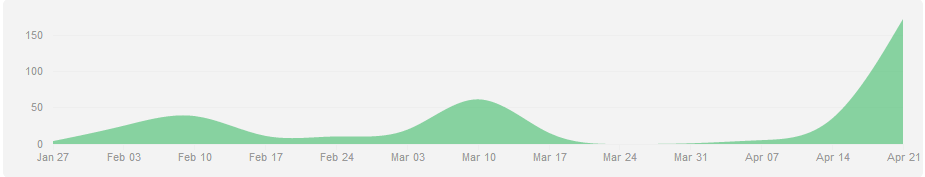
\includegraphics{{images/graph-commits.png}}
	\caption{An graph of contributions to the github repository over time.}
	\label{img-commitgraphs}
\end{figure}

\part{Conclusion}

%``And so we find ourselves standing here, at the end of it all, gazing upon the work which has been done.''
The finished program is capable of playing different sounds when different buttons are pushed; including three different sound effects and one start-up melody.
It is also capable of playing modfiles, represented as an array of integers.
Measures taken to increase the energy efficiency of the program resulted in a reduction of the quality of the sounds, illustrating that energy efficiency cannot always be achieved without sacrifice.
The authors feel the assignment has further increased their proficiency and familiarity with C and hardware-level programming, as well as sound theory.
In conclusion, the project was completed according to the specifications within the given timeframe.
In the world of business, this is commonly known as ``great success''.

\begin{center}
A video demonstration of the solution program running on an STK1000 can be seen at \\
\url{http://www.youtube.com/watch?v=cdKfN6vJjk8}
\end{center}


\newpage

\bibliography{bibtexlibz}{}
\bibliographystyle{plain}
\nocite{*}
All internet resources were checked on \today.
\end{document}
